\documentclass[oneside,letterpaper]{scrartcl}
\usepackage[utf8]{inputenc}
\usepackage[pdftex]{graphicx}
\usepackage{hyperref}
\usepackage{fullpage}
\usepackage{alltt}

%\setcounter{secnumdepth}{-1}
\newcommand{\secref}[1]{\S \ref{#1}, pg. \pageref{#1}}

\title{Reshaping data with the {\tt reshape} package}
%\VignetteIndexEntry{An introduction to reshaping data with reshape}
\author{Hadley Wickham. \\
\url{http://had.co.nz/reshape}}

\date{September 2006}

\usepackage{/Library/Frameworks/R.framework/Resources/share/texmf/Sweave}
\begin{document}

\maketitle
\setcounter{tocdepth}{2}
\tableofcontents
\newpage

\section{Introduction}

% decumar<<< 
% smiths <- data.frame(subject = c("John Smith", "Mary Smith"), time = as.integer(1), age = c(33, NA), weight=c(90, NA), height=c(1.87, 1.54))
% library(ggplot)
% library(xtable)
% >>>

Reshaping data is a common task in practical data analysis, and it is usually tedious and unintuitive.  

Data often has multiple levels of grouping (nested treatments, split plot designs, or repeated measurements) and typically requires investigation at multiple levels. For example, from a long term clinical study we may be interested in investigating summarising patients, treatments, trends over time or combinations of each. Performing these investigations fluently requires the data to be reshaped in different ways, but most software packages make it difficult to generalise these tasks and code needs to be written for each specific case. 

While most practitioners are intuitively familiar with the idea of reshaping, it is useful define it a little more formally.  Data reshaping is easiest to define with respect to aggregation.  Aggregation is a common and familiar task where data is reduced and rearranged into a smaller, more convenient form, with a concomitant reduction in the amount of information.  One commonly used aggregation tool is Excel's Pivot tables.  Reshaping involves a similar rearrangement, but preserves all original information; where aggregation reduces many cells in the original data set to one cell in the new dataset, reshaping preserves a one-to-one connection.   These ideas are expanded and formalised in the next section. 

In R, there are a number of general functions that can aggregate data, for example {\tt tapply}, {\tt by} and {\tt aggregate}, and a function specifically for reshaping data, {\tt reshape}.  Each of these functions deals well with one or two specific scenarios, and each requires slightly different input arguments.  In practice, careful thought is required to piece together the correct sequence of operations to get your data into the form that you want.  The {\tt reshape} package overcomes these problems with a general conceptual framework that needs just two functions: {\tt melt} and {\tt cast}.

This document introduces to the conceptual framework of melting and casting, \S \ref{sec:framework}, then provides a detailed description of each with plenty of examples, \S \ref{sec:melt} and \ref{sec:cast}.  The {\tt reshape} package also provides a number of convenience functions for general data manipulation, described in \S \ref{sec:convenience}. The paper concludes with case studies using melt and cast in real life examples, \S \ref{sec:case-studies}.

\newpage
\section{Conceptual framework}\label{sec:framework}

To help us think about the many ways we might rearrange a data set it is useful to think about data in a new way.  Usually, we think about data in terms of a matrix or data frame, where we have observations in the rows and variables in the columns.  For the purposes of reshaping, we can divide the variables into two groups: identifier and measured variables.

\begin{enumerate}
	\item Identifier, or id, variables identify the unit that measurements take place on.  Id variables are usually discrete, and are typically fixed by design.  In ANOVA notation ($Y_{ijk}$), id variables are the indices on the variables ($i, j, k$).  In database terminology, these are the primary keys.
	\item Measured variables represent what attributes measured on each unit ($Y$).
\end{enumerate}

\noindent It is possible to take this abstraction a step further and say there are only id variables and a value, where the id variables also identify what measured variable the value represents.  For example, we could represent this data set, which has two id variables, subject and time, 

\bigskip

% decumar<<< 
% print(xtable(smiths, align="|r|l|r||r|r|r|", digits=rep(0,6)), floating=FALSE)
% |||
% latex table generated in R 2.4.0 by xtable 1.3-2 package
% Wed Sep 27 12:57:16 2006
\begin{tabular}{|r|l|r||r|r|r|}
\hline
 & subject & time & age & weight & height \\
\hline
1 & John Smith & 1 & 33 & 90 & 2 \\
2 & Mary Smith & 1 &  &  & 2 \\
\hline
\end{tabular}
% >>>

\bigskip
\noindent as:
\bigskip

% decumar<<< 
% smithsm <- melt(smiths, id=c("subject", "time"), preserve.na=FALSE)
% print(xtable(smithsm, align="|l|l|r|l||r|", digits=c(rep(0,4),2)), floating=FALSE)
% |||
% latex table generated in R 2.4.0 by xtable 1.3-2 package
% Wed Sep 27 12:57:16 2006
\begin{tabular}{|l|l|r||l|r|}
\hline
 & subject & time & variable & value \\
\hline
1 & John Smith & 1 & age & 33 \\
2 & John Smith & 1 & weight & 90 \\
3 & John Smith & 1 & height & 2 \\
4 & Mary Smith & 1 & height & 2 \\
\hline
\end{tabular}
% >>>

\bigskip
\noindent where each row represents one observation of one variable.  This operation is called {\bf melting} and produces ``molten'' data.  Compared to the original data set, it has a new id variable ``variable'', and a new column ``value'', which represents the value of that observation.  We now have the data in a form in which there are only id variables and a value.

From this form, we can create new forms by specifying which variables should form the columns and rows.  This operating is called {\bf casting}.  In the original data frame, the ``variable'' id variable forms the columns, and all identifiers form the rows.  We don't have to specify all the original id variables in the new form.  When we don't, the id variables no longer uniquely identify one row, and in this case we need a function that reduces these many numbers to one.  This is called an aggregation function. 

The following section continues with the example and describes the melting operation in detail with an implementation in R.

\newpage
\section{Melting data}\label{sec:melt}

Melting a data frame is a little trickier in practice than it is in theory.  This section describes the practical use of the {\tt melt} function in R.

The {\tt melt} function needs to know which variables are measured and which are identifiers.  This distinction should be obvious from your design: if you fixed the value, it is an id variable.  If you don't specify the variables explicitly, {\tt melt} will assume that any factor or integer column is an id variable.  If you specify only one of measured and identifier variables, {\tt melt} assumes that all the other variables are the other sort.  For example, with the {\tt smiths} dataset, as used in the previous section, all the following calls have the same effect:

\begin{alltt}
melt(smiths, id=c("subject","time"), measured=c("age","weight","height"))
melt(smiths, id=c("subject","time"))
melt(smiths, id=1:2)
melt(smiths, measured=c("age","weight","height"))
melt(smiths)
\end{alltt}

% decumar<<< 
% interweave({
% melt(smiths)
% })
% |||
\begin{alltt}
> melt(smiths)
     subject time variable value
1 John Smith    1      age  33.0
2 Mary Smith    1      age    NA
3 John Smith    1   weight  90.0
4 Mary Smith    1   weight    NA
5 John Smith    1   height   1.9
6 Mary Smith    1   height   1.5

\end{alltt}
% >>>

Melt doesn't make many assumptions about your measured and id variables: there can be any number, in any order, and the values within the columns can be in any order too.  You do, however, need to ensure there are no missing values in id variables.  There is only one assumption that {\tt melt} makes: all measured values must be of the same type.  This is usually ok, because most of the time measured variables are numeric, but unfortunately if you are working with measured variables of different types, you will need to split them intop separate data frames.

\subsection{Melting data with id variables encoded in column names}\label{sub:multiple-identifiers}

A more complicated case is where the variable names contain information about more than one variable.  For example, here we have an experiment with two treatments (A and B) with data recorded on two time points (1 and 2), and the column names represent both treatment and time.

% decumar<<< 
% interweave({
% trial <- data.frame(id=factor(1:4), A1=c(1,2,1,2), A2=c(2,1,2,1), B1=c(3,3,3,3))
% (trialm <- melt(trial))
% })
% |||
\begin{alltt}
> trial <- data.frame(id = factor(1:4), A1 = c(1, 2, 1, 2), A2 = c(2, 
+     1, 2, 1), B1 = c(3, 3, 3, 3))
> (trialm <- melt(trial))
   id variable value
1   1       A1     1
2   2       A1     2
3   3       A1     1
4   4       A1     2
5   1       A2     2
6   2       A2     1
7   3       A2     2
8   4       A2     1
9   1       B1     3
10  2       B1     3
11  3       B1     3
12  4       B1     3

\end{alltt}
% >>>

To fix this we need to create a time and treatment column after reshaping:

% decumar<<< 
% interweave({
% (trialm <- cbind(trialm, colsplit(trialm$variable, names=c("treatment", "time"))))
% })
% |||
\begin{alltt}
> (trialm <- cbind(trialm, colsplit(trialm$variable, names = c("treatment", 
+     "time"))))
   id variable value treatment time
1   1       A1     1         A    1
2   2       A1     2         A    1
3   3       A1     1         A    1
4   4       A1     2         A    1
5   1       A2     2         A    2
6   2       A2     1         A    2
7   3       A2     2         A    2
8   4       A2     1         A    2
9   1       B1     3         B    1
10  2       B1     3         B    1
11  3       B1     3         B    1
12  4       B1     3         B    1

\end{alltt}
% >>>

I'm not aware of any general way to do this, so you may need to modify the code in {\tt colsplit} depending on your situation. 

\subsection{Melting arrays}\label{sub:arrays}

Sometimes, especially if your data is highly balanced or crossed, the data you want to reshape may be stored in an {\tt array}.  In this case, each array index acts as an id variable, and the value in the cell is the measured value.  The melt method uses the {\tt dimnames} component to determine the names and values of the id variables, as shown in this example:

% decumar<<< 
% interweave({
% (a <- array(sample(1:6), c(3,2,1)))
% melt(a)
% dimnames(a) <- lapply(dim(a), function(x) LETTERS[1:x])
% melt(a)
% names(dimnames(a)) <- c("trt", "loc", "time")
% melt(a)
% })
% |||
\begin{alltt}
> (a <- array(sample(1:6), c(3, 2, 1)))
, , 1

     [,1] [,2]
[1,]    6    3
[2,]    2    4
[3,]    1    5


> melt(a)
  X1 X2 X3 value
1  1  1  1     6
2  2  1  1     2
3  3  1  1     1
4  1  2  1     3
5  2  2  1     4
6  3  2  1     5

> dimnames(a) <- lapply(dim(a), function(x) LETTERS[1:x])
> melt(a)
  X1 X2 X3 value
1  A  A  A     6
2  B  A  A     2
3  C  A  A     1
4  A  B  A     3
5  B  B  A     4
6  C  B  A     5

> names(dimnames(a)) <- c("trt", "loc", "time")
> melt(a)
  trt loc time value
1   A   A    A     6
2   B   A    A     2
3   C   A    A     1
4   A   B    A     3
5   B   B    A     4
6   C   B    A     5

\end{alltt}
% >>>

\subsection{Missing values in molten data}\label{sub:missing_values}

Finally, it's important to discuss what happens to missing values when you melt your data.  Explicitly coded missing values usually denote sampling zeros rather than structural missings, which are usually implicit in the data.  Clearly a structural missing depends on the structure of the data and as we are changing the structure of the data, we might expect some changes to structural missings.  Structural missings change from implicit to explicit when we change from a nested to a crossed structure.  For example, imagine a dataset with two id variables, sex (male or female) and pregnant (yes or no).  When the variables are nested (ie. both on the same dimension) then the missing value ``pregnant male'' is encoded by its absence.  However, in a crossed view, we need to add an explicit missing as there will now be a cell which must be filled with something.  This is illustrated below.

% decumar<<< 
% preg <- data.frame(sex=c("male", "female","female"), pregnant=c("no", "no", "yes"), value=c(10,14,4))
% xtable(preg)
% |||
% latex table generated in R 2.4.0 by xtable 1.3-2 package
% Wed Sep 27 12:57:17 2006
\begin{table}[ht]
\begin{center}
\begin{tabular}{rllr}
\hline
 & sex & pregnant & value \\
\hline
1 & male & no & 10.00 \\
2 & female & no & 14.00 \\
3 & female & yes & 4.00 \\
\hline
\end{tabular}
\end{center}
\end{table}
% >>>

% decumar<<< 
% xtable(cast(preg, sex ~ pregnant))
% |||
% latex table generated in R 2.4.0 by xtable 1.3-2 package
% Wed Sep 27 12:57:17 2006
\begin{table}[ht]
\begin{center}
\begin{tabular}{rlrr}
\hline
 & sex & no & yes \\
\hline
1 & female & 14.00 & 4.00 \\
2 & male & 10.00 &  \\
\hline
\end{tabular}
\end{center}
\end{table}
% >>>

Continuing along this path, the molten form is a perfectly nested form: there are no crossings.  For this reason, it is possible to encode all missing values implicitly (by omitting that combination of id variables) rather than explicitly (with an {\tt NA} value).

However, you may expect these to be in the data frame, and it is a bad idea for a function to throw data away by default, so you need to explicitly state that implicit missing values are ok.  In most cases it is safe to get rid of them, which you can do by using {\tt preserve.na = FALSE} in the call to {\tt melt}.  The two different results are illustrated below.

% decumar<<< 
% interweave({
% melt(smiths)
% melt(smiths, preserve.na = FALSE)
% })
% |||
\begin{alltt}
> melt(smiths)
     subject time variable value
1 John Smith    1      age  33.0
2 Mary Smith    1      age    NA
3 John Smith    1   weight  90.0
4 Mary Smith    1   weight    NA
5 John Smith    1   height   1.9
6 Mary Smith    1   height   1.5

> melt(smiths, preserve.na = FALSE)
     subject time variable value
1 John Smith    1      age  33.0
2 John Smith    1   weight  90.0
3 John Smith    1   height   1.9
4 Mary Smith    1   height   1.5

\end{alltt}
% >>>
 
If you don't use {\tt preserve.na = FALSE} you will need to make sure to account for possible missing values when aggregating (\secref{sub:aggregation}), for example, by supplying {\tt na.rm = TRUE} to {\tt mean}, {\tt sum} and {\tt var}.

\newpage
\section{Casting molten data}\label{sec:cast}

Once you have your data in the molten form, you can use {\tt cast} to create the form you want.  {\tt Cast} has two arguments that you will always supply:

\begin{itemize}
	\item {\tt data}: the molten data set to cast
	\item {\tt formula}: the casting formula which describes the shape of the output format (if you omit this argument, cast will return the data frame to its pre-molten form)
\end{itemize} 

This section explains the different casting formulas you can use.  It also explains the use of the other optional arguments to cast:

\begin{itemize}
	\item {\tt fun.aggregate}: aggregation function to use (if necessary)
	\item {\tt margins}: what marginal values should be computed
	\item {\tt subset}: only operate on a subset of the original data.
\end{itemize}

\subsection{Basic use}\label{sub:basic_use}

The casting formula has the following basic form: {\tt col\_var\_1 +  col\_var\_2 $\sim$ row\_var\_1 + row\_var\_2}.  This describes which variables you want to appear in the columns and which in the rows.  These variables need to come from the molten data frame or be one of the following special variables:

\begin{itemize}
	\item {\tt .} corresponds to no variable, useful when creating formulas of the form {\tt .\ $\sim$ x} or {\tt x $\sim$ .}
	\item {\tt ...} represents all variables not previously included in the casting formula.  Including this in your formula will guarantee that no aggregation occurs.  There can be only one {\tt ...} in a cast formula.
	\item {\tt result\_variable} is used when your aggregation formula returns multiple results.  See \secref{sub:multiple_returns} for more details.
\end{itemize}

The first set of examples illustrate reshaping: all the original variables are retained in the new form.  Each of these reshaping changes which of the identifier variables appear in the columns and which in the rows.  The typical view of a data frame has the ``variable'' variable in the columns and all others in the rows, but if we were interested in investigating the relationships between subjects or times, we might put those in the columns instead.

% decumar<<< 
% interweave({
% cast(smithsm, time + subject ~ variable)
% cast(smithsm, ... ~ variable)
% cast(smithsm, ... ~ subject)
% cast(smithsm, ... ~ time)
% })
% |||
\begin{alltt}
> cast(smithsm, time + subject ~ variable)
  time    subject age weight height
1    1 John Smith  33     90    1.9
2    1 Mary Smith  NA     NA    1.5

> cast(smithsm, ... ~ variable)
     subject time age weight height
1 John Smith    1  33     90    1.9
2 Mary Smith    1  NA     NA    1.5

> cast(smithsm, ... ~ subject)
  time variable John.Smith Mary.Smith
1    1      age       33.0         NA
2    1   weight       90.0         NA
3    1   height        1.9        1.5

> cast(smithsm, ... ~ time)
     subject variable   X1
1 John Smith      age 33.0
2 John Smith   weight 90.0
3 John Smith   height  1.9
4 Mary Smith   height  1.5

\end{alltt}
% >>>

The following examples demonstrate aggregation.  See \secref{sub:aggregation} for more details.  These examples use the french fries dataset included in the {\tt reshape} package.  The first few rows are shown in \ref{tbl:ff}.  It is data from a sensory experiment on french fries, where different types of frier oil, {\tt treatment}, were tested by different people, {\tt subject}, over ten weeks {\tt time}.

% decumar<<<
% xtable(head(french_fries), label="tbl:ff", caption="Sample of french fries dataset")
% |||
% latex table generated in R 2.4.0 by xtable 1.3-2 package
% Wed Sep 27 12:57:22 2006
\begin{table}[ht]
\begin{center}
\begin{tabular}{rlllrrrrrr}
\hline
 & time & treatment & subject & rep & potato & buttery & grassy & rancid & painty \\
\hline
61 & 1 & 1 & 3 & 1.00 & 2.90 & 0.00 & 0.00 & 0.00 & 5.50 \\
25 & 1 & 1 & 3 & 2.00 & 14.00 & 0.00 & 0.00 & 1.10 & 0.00 \\
62 & 1 & 1 & 10 & 1.00 & 11.00 & 6.40 & 0.00 & 0.00 & 0.00 \\
26 & 1 & 1 & 10 & 2.00 & 9.90 & 5.90 & 2.90 & 2.20 & 0.00 \\
63 & 1 & 1 & 15 & 1.00 & 1.20 & 0.10 & 0.00 & 1.10 & 5.10 \\
27 & 1 & 1 & 15 & 2.00 & 8.80 & 3.00 & 3.60 & 1.50 & 2.30 \\
\hline
\label{tbl:ff}
\end{tabular}
\end{center}
\end{table}
% >>>

The most severe type of aggregation is reducing an entire table to one number.  This is what happens when you use the cast formula $. \sim .$ 

% decumar<<< 
% interweave({
% ffm <- melt(french_fries, id=1:4, preserve=FALSE)
% cast(ffm, . ~ ., length)
% })
% |||
%>>>

The next example produces a summary for each treatment.  We can get the same results using {\tt taply}, or for the special case of {\tt length}, table.  The disadvantage of these methods is their lack of generality -- they can only produce certain ``shapes'' of data.

% decumar<<< 
% interweave({
% cast(ffm, treatment ~ ., length)
% tapply(ffm$value, ffm$treatment, length)
% table(ffm$treatment)
% cast(ffm, treatment ~ ., sum)
% tapply(ffm$value, ffm$treatment, sum)
% })
% |||
%>>>

Here are some more examples illustrating the effects of changing the order ad position of variables in the cast formula.  Each of these examples displays exactly the same data, just arranged in a slightly different form.  When thinking about how to arrange your data, think about which comparisons are most important.

% decumar<<< 
% interweave({
% cast(ffm, rep ~ treatment, length)
% table(ffm$rep, ffm$treatment)
% cast(ffm, treatment ~ rep, length)
% table(ffm$treatment, ffm$rep)
% cast(ffm, treatment + rep ~ ., length)
% ftable(ffm[c("treatment", "rep")], row.vars=1:2)
% cast(ffm, rep + treatment ~ ., length)
% cast(ffm, . ~ treatment + rep, length)
% })
% |||
\begin{alltt}
> ffm <- melt(french_fries, id = 1:4, preserve = FALSE)
> cast(ffm, . ~ ., length)
  value value.1
1 value    3471

> cast(ffm, treatment ~ ., length)
  treatment value
1         1  1159
2         2  1157
3         3  1155

> cast(ffm, . ~ treatment, length)
  value   X1   X2   X3
1 value 1159 1157 1155

> cast(ffm, rep ~ treatment, length)
  rep  X1  X2  X3
1   1 579 578 575
2   2 580 579 580

> cast(ffm, treatment ~ rep, length)
  treatment  X1  X2
1         1 579 580
2         2 578 579
3         3 575 580

> cast(ffm, treatment + rep ~ ., length)
  treatment rep value
1         1   1   579
2         1   2   580
3         2   1   578
4         2   2   579
5         3   1   575
6         3   2   580

> cast(ffm, rep + treatment ~ ., length)
  rep treatment value
1   1         1   579
2   1         2   578
3   1         3   575
4   2         1   580
5   2         2   579
6   2         3   580

> cast(ffm, . ~ treatment + rep, length)
  value X1_1 X1_2 X2_1 X2_2 X3_1 X3_2
1 value  579  580  578  579  575  580

\end{alltt}
% >>>

As illustrated above, the order in which the row and column variables are specified in is very important.  As with a contingency table there are many possible ways of displaying the same variables, and the way they are organised reveals different patterns in the data.  Variables specified first vary slowest, and those specified last vary fastest.  Because comparisons are made most easily between adjacent cells, the variable you are most interested in should be specified last, and the early variables should be thought of as conditioning variables.  An additional constraint is that displays have limited width but essentially infinite length, so variables with many levels must be specified as row variables.  

\subsection{Aggregation}\label{sub:aggregation}

Whenever there are fewer cells in the cast form than there were in the original data format, an aggregation function is necessary.  This formula reduces multiple cells into one, and is supplied in the {\tt fun.aggregate} argument, which defaults (with a warning) to {\tt length}.  Aggregation is a very common and useful operation and the case studies section (\secref{sec:case_studies}) contains many other examples of aggregation.  

The aggregation function will be passed the vector of values for one cell.  It may take other arguments, passed in through {\tt ...} in {\tt cast}.  Here are a few examples:

% decumar<<< 
% interweave({
% cast(ffm, . ~ treatment)
% cast(ffm, . ~ treatment, function(x) length(x))
% cast(ffm, . ~ treatment, length)
% cast(ffm, . ~ treatment, sum)
% cast(ffm, . ~ treatment, mean)
% cast(ffm, . ~ treatment, mean, trim=0.1)
% })
% |||
\begin{alltt}
> cast(ffm, . ~ treatment)
Warning:  Aggregation requires fun.aggregate: length used as default 
  value   X1   X2   X3
1 value 1159 1157 1155

> cast(ffm, . ~ treatment, function(x) length(x))
  value   X1   X2   X3
1 value 1159 1157 1155

> cast(ffm, . ~ treatment, length)
  value   X1   X2   X3
1 value 1159 1157 1155

> cast(ffm, . ~ treatment, sum)
  value   X1   X2   X3
1 value 3702 3640 3640

> cast(ffm, . ~ treatment, mean)
  value  X1  X2  X3
1 value 3.2 3.1 3.2

> cast(ffm, . ~ treatment, mean, trim = 0.1)
  value  X1  X2  X3
1 value 2.6 2.5 2.6

\end{alltt}
% >>>


\subsection{Margins}\label{sub:margins}

It's often useful to be able to add margins to your tables.  What is a margin?  It is marginal in the statistical sense: we have averaged over the other variables.  You can tell {\tt cast} to display all margins with {\tt margins = TRUE}, or list individual variables in a character vector, {\tt margins=c("subject","day")}.  There are two special margins, {\tt "grand\_col"} and {\tt "grand\_row"}, which display margins for the overall columns and rows respectively. Margins are displayed with a ``.'' instead of the value of the variable. 

These examples illustrate some of the possible ways to use margins.  I've used sum as the aggregation function so that you can check the results yourself. Note that changing the order and position of the variables in the cast formula affects the margins that appear.  

% decumar<<< 
% interweave({
% cast(ffm, treatment ~ ., sum, margins=TRUE)
% cast(ffm, treatment ~ ., sum, margins="grand_row")
% cast(ffm, treatment ~ rep, sum, margins=TRUE)
% cast(ffm, treatment + rep ~ . , sum, margins=TRUE)
% cast(ffm, treatment + rep ~ time , sum, margins=TRUE)
% cast(ffm, treatment + rep ~ time , sum, margins="treatment")
% cast(ffm, rep + treatment ~ time , sum, margins="rep")
% })
% |||
\begin{alltt}
> cast(ffm, treatment ~ ., sum, margins = TRUE)
  treatment value
1         1  3702
2         2  3640
3         3  3640

> cast(ffm, treatment ~ ., sum, margins = "grand_row")
  treatment value
1         1  3702
2         2  3640
3         3  3640

> cast(ffm, treatment ~ rep, sum, margins = TRUE)
  treatment   X1   X2     .
1         1 1857 1845  3702
2         2 1836 1804  3640
3         3 1739 1901  3640
4      <NA> 5433 5550 10983

> cast(ffm, treatment + rep ~ ., sum, margins = TRUE)
  treatment rep value
1         1   1  1857
2         1   2  1845
3         1  NA  3702
4         2   1  1836
5         2   2  1804
6         2  NA  3640
7         3   1  1739
8         3   2  1901
9         3  NA  3640

> cast(ffm, treatment + rep ~ time, sum, margins = TRUE)
   treatment rep   X1   X2   X3   X4   X5   X6   X7   X8  X9  X10     .
1          1   1  156  213  206  181  208  182  156  185 176  194  1857
2          1   2  216  195  194  154  204  185  158  216 122  201  1845
3          1  NA  373  408  400  335  412  366  314  402 298  396  3702
4          2   1  187  213  172  193  157  183  175  173 185  199  1836
5          2   2  168  157  186  187  173  215  172  189 145  212  1804
6          2  NA  355  370  358  380  330  398  347  362 330  411  3640
7          3   1  189  212  172  190  151  161  165  150 173  175  1739
8          3   2  217  180  199  192  183  192  218  175 164  182  1901
9          3  NA  406  392  372  382  334  353  384  325 337  357  3640
10      <NA>  NA 1134 1170 1129 1097 1076 1117 1045 1088 965 1163 10983

> cast(ffm, treatment + rep ~ time, sum, margins = "treatment")
  treatment rep  X1  X2  X3  X4  X5  X6  X7  X8  X9 X10
1         1   1 156 213 206 181 208 182 156 185 176 194
2         1   2 216 195 194 154 204 185 158 216 122 201
3         1  NA 373 408 400 335 412 366 314 402 298 396
4         2   1 187 213 172 193 157 183 175 173 185 199
5         2   2 168 157 186 187 173 215 172 189 145 212
6         2  NA 355 370 358 380 330 398 347 362 330 411
7         3   1 189 212 172 190 151 161 165 150 173 175
8         3   2 217 180 199 192 183 192 218 175 164 182
9         3  NA 406 392 372 382 334 353 384 325 337 357

> cast(ffm, rep + treatment ~ time, sum, margins = "rep")
  rep treatment  X1  X2  X3  X4  X5  X6  X7  X8  X9 X10
1   1         1 156 213 206 181 208 182 156 185 176 194
2   1         2 187 213 172 193 157 183 175 173 185 199
3   1         3 189 212 172 190 151 161 165 150 173 175
4   1      <NA> 532 637 550 564 515 526 497 509 534 568
5   2         1 216 195 194 154 204 185 158 216 122 201
6   2         2 168 157 186 187 173 215 172 189 145 212
7   2         3 217 180 199 192 183 192 218 175 164 182
8   2      <NA> 601 533 579 533 560 591 548 580 430 595

\end{alltt}
% >>>

\subsection{Returning multiple values}\label{sub:multiple_returns}

Occasionally it is useful to aggregate with a function that returns multiple values, e.g.\ {\tt range} or {\tt summary}.  This can be thought of as combining multiple {\tt cast}s each with an aggregation function that returns one variable.  To display this we need to add an extra variable, {\tt result\_variable} that differentiates the multiple return values.   By default, this new id variable will be shown as the last column variable, but you can specify the position manually by including {\tt result\_variable} in the casting formula.

% decumar<<< 
% interweave({
% cast(ffm, treatment ~ ., summary)
% cast(ffm, treatment ~ ., quantile, c(0.05, 0.5, 0.95))
% cast(ffm, treatment ~ rep, range)
% named.range <- function(x) c(min=min(x), max=max(x))
% cast(ffm, treatment ~ rep, named.range)
% cast(ffm, treatment ~ result_variable + rep, named.range)
% cast(ffm, treatment ~ rep ~ result_variable, named.range)
% })
% |||
\begin{alltt}
> cast(ffm, treatment ~ ., summary)
  treatment Min. X1st.Qu. Median Mean X3rd.Qu. Max.
1         1    0        0    1.6  3.2      5.4   15
2         2    0        0    1.4  3.1      5.4   15
3         3    0        0    1.5  3.1      5.7   14

> cast(ffm, treatment ~ ., quantile, c(0.05, 0.5, 0.95))
  treatment X5. X50. X95.
1         1   0  1.6   11
2         2   0  1.4   11
3         3   0  1.5   11

> cast(ffm, treatment ~ rep, range)
  treatment X1_X1 X1_X2 X2_X1 X2_X2
1         1     0    15     0    14
2         2     0    15     0    14
3         3     0    14     0    14

> named.range <- function(x) c(min = min(x), max = max(x))
> cast(ffm, treatment ~ rep, named.range)
  treatment X1_min X1_max X2_min X2_max
1         1      0     15      0     14
2         2      0     15      0     14
3         3      0     14      0     14

> cast(ffm, treatment ~ result_variable + rep, named.range)
  treatment min_1 min_2 max_1 max_2
1         1     0     0    15    14
2         2     0     0    15    14
3         3     0     0    14    14

> cast(ffm, treatment ~ rep ~ result_variable, named.range)
, , 1

  [,1] [,2]
1    0    0
2    0    0
3    0    0

, , 2

  [,1] [,2]
1   15   14
2   15   14
3   14   14


\end{alltt}
% >>>

Using an aggregation function that returns multidimensional objects (eg. matrices or arrays) does not work.  You may be able to work around this deficiency by creating a high-D array, and then using {\tt iapply}.

\subsection{High-dimensional arrays}\label{sub:high_dimensional_arrays}

You can use more than one $\sim$ to create structures with more than two dimensions.  For example, a cast formula of {\tt x $\sim$ y $\sim$ z} will create a 3D array with x, y, and z dimensions. You can still use multiple variables in each dimension: {\tt x + a $\sim$ y + b $\sim$ z + c}.  The following example shows the resulting dimensionality of various casting formulas (I don't show the actual output for examples because it would be too large.  You may want to verify the results for yourself):

% decumar<<< 
% interweave({
% options(digits=2)
% dim(cast(ffm, time ~ variable ~ treatment, mean))
% dim(cast(ffm, time ~ variable ~ treatment + rep, mean))
% dim(cast(ffm, time ~ variable ~ treatment ~ rep, mean))
% dim(cast(ffm, time ~ variable ~ subject ~ treatment ~ rep))
% dim(cast(ffm, time ~ variable ~ subject ~ treatment ~ result_variable, range))
% })
% |||
\begin{alltt}
> dim(cast(ffm, time ~ variable ~ treatment, mean))
[1] 10  5  3

> dim(cast(ffm, time ~ variable ~ treatment + rep, mean))
[1] 10  5  6

> dim(cast(ffm, time ~ variable ~ treatment ~ rep, mean))
[1] 10  5  3  2

> dim(cast(ffm, time ~ variable ~ subject ~ treatment ~ rep))
[1] 10  5 12  3  2

> dim(cast(ffm, time ~ variable ~ subject ~ treatment ~ result_variable, 
+     range))
[1] 10  5 12  3  2

\end{alltt}
% >>>

The high-dimensional array form is useful for sweeping out margins with {\tt sweep}, or modifying with {\tt iapply} (\secref{ssub:idempotent_apply}).  See the case studies for examples.  

The $\sim$ operator is a type of crossing operator, as all combinations of the variables will appear in the output table.   Compare this to the $+$ operator, where only combinations that appear in the data will appear in the output.  For this reason, increasing the dimensionality of the output, i.e.\ using more $\sim$s, will generally increase the number of (structural) missings.  This is illustrated in the next example:

% decumar<<< 
% ffm <- melt(french_fries, id=1:4, preserve=FALSE)
% interweave({
% sum(is.na(cast(ffm, ... ~ . )))
% sum(is.na(cast(ffm, ... ~ rep)))
% sum(is.na(cast(ffm, ... ~ subject)))
% sum(is.na(cast(ffm, ... ~ time ~ subject ~ variable ~ rep)))
% })
% |||
\begin{alltt}
> sum(is.na(cast(ffm, ... ~ .)))
[1] 0

> sum(is.na(cast(ffm, ... ~ rep)))
[1] 9

> sum(is.na(cast(ffm, ... ~ subject)))
[1] 129

> sum(is.na(cast(ffm, ... ~ time ~ subject ~ variable ~ rep)))
[1] 129

\end{alltt}
% >>>

Margins currently do not work with high-dimensional arrays.  

\subsection{Lists}\label{sub:lists}

You can also use {\tt cast} to produce lists.  This is done with the $|$ operator. Using multiple variables after $|$ will create multiple levels of nesting.

% decumar<<< 
% interweave({
% cast(ffm, treatment ~ rep | variable, mean)
% cast(ffm, . ~ variable | rep, mean)
% varrep <- cast (ffm, . ~ time | variable + rep, mean)
% varrep$painty
% varrep$painty$`2`
% })
% |||
\begin{alltt}
> cast(ffm, treatment ~ rep | variable, mean)
$potato
  treatment  X1  X2
1         1 6.8 7.0
2         2 7.2 6.8
3         3 6.9 7.0

$buttery
  treatment  X1  X2
1         1 1.8 1.8
2         2 2.0 2.0
3         3 1.8 1.6

$grassy
  treatment   X1   X2
1         1 0.45 0.85
2         2 0.69 0.64
3         3 0.59 0.77

$rancid
  treatment  X1  X2
1         1 4.3 3.8
2         2 3.7 3.5
3         3 3.8 4.0

$painty
  treatment  X1  X2
1         1 2.7 2.4
2         2 2.3 2.6
3         3 2.0 3.0


> length(cast(ffm, treatment ~ rep | variable, mean))
[1] 5

> length(cast(ffm, treatment ~ rep | subject, mean))
[1] 12

> length(cast(ffm, treatment ~ rep | time, mean))
[1] 10

> sapply(cast(ffm, treatment ~ rep | time + variable, mean), length)
 1  2  3  4  5  6  7  8  9 10 
 5  5  5  5  5  5  5  5  5  5 

\end{alltt}
% >>>

This form is useful for input to {\tt lapply} and {\tt sapply}, and completes the discussion of the different types of output you can create with reshape.

%\subsection{Subsetting}\label{sub:subsetting}
%
%It's possible to subset as part of reshaping.  You do this with the {\tt subset} argument, which takes a logical vector.
%
%Example goes here.
%
%\subsection{Row and column names}
%
%There are two ways to think about the results from an aggregation command, as either a matrix of numbers with some attributes that describe the row and column names, or as a data frame with the row names as columns.  Most current R aggregation functions return the first, implicit, form, whereas cast returns the explicit data frame form.  Why the difference?  The implicit form is often inconvenient to deal with---rownames are data too.
%
%Two forms, how to change between them.

%\newpage
%\section{Stamping molten data}\label{sec:stamping_molten_data}
%
%When aggregating, your aggregation function operates on vectors of data, of just the measured values.  Stamp is very except instead of passing the measured values to the aggregation function, the entire data frame (containing both measured values and id variables) is passed instead.  This allows you to do things like you could with the {\tt by} or {\tt tapply} functions in base R, except the results will be arranged in a nicer form, like aggregated data.
%
%Stamp makes it easy to look at multivariate summaries for subsets of your data.

\newpage
\section{Other convenience functions}\label{sec:convenience}

There are many other problems encountered in practical analysis that can be painful to overcome with out some handy functions.  This section describes some of the functions that reshape provides to make dealing with data a little bit easier.  

\subsection{Factors}\label{sub:factor_related}

\begin{itemize}
	\item {\tt combine\_factor} combines levels in a factor.  For example, if you have many small levels you can combine them together into an ``other'' level.
	
% decumar<<< 
% interweave({
% (f <- factor(letters[1:5]))
% combine_factor(f, c(1, 2, 3, 3, 3))
% combine_factor(f, c(1, 2))
% })
% |||
% >>>
	
	\item {\tt reorder\_factor} reorders a factor based on another variable.  For example, you can order a factor by the average value of a variable for each level.

% decumar<<< 
% interweave({
% df <- data.frame(a=letters[sample(5, 15, replace=TRUE)], y=rnorm(15))
% (f <- reorder_factor(df$a, tapply(df$y, df$a, mean)))
% (f <- reorder_factor(df$a, tapply(df$y, df$a, length)))
% })
% |||
% >>>

\end{itemize}

\subsection{Data frames}\label{sub:data_related}

\begin{itemize}
	\item {\tt rescaler} performs column-wise rescaling of data frames,  with a variety of different scaling options including rank, common range and common variance.  It automatically preserves non-numeric variables.
	\item {\tt merge.all} merges multiple data frames together, an extension of {\tt merge} in base R.  It assumes that all columns with the same name should be equated.
	\item {\tt rbind.fill} {\tt rbind}s two data frames together, filling in any missing columns in the second data frame with missing values.
\end{itemize}

\subsection{Miscellaneous}\label{sub:miscellaneous}

\begin{itemize}
	\item {\tt round\_any} allows you to round a number to any degree of accuracy, e.g.\ to the nearest 1, 10, or any other number. 
	
% decumar<<< 
% interweave({
% round_any(105, 10)
% round_any(105, 4)
% round_any(105, 4, ceiling)
% |||
% >>>	

	\item {\tt iapply} is an idempotent version of the {\tt apply} function.  This is useful when dealing with high-dimensional arrays as it will return the array in the same shape that you sent it.  It also supports functions that return matrices or arrays in a sensible manner.
\end{itemize}

\newpage
\section{Case studies}\label{sec:case-studies}

These case studies provide fuller exposition of using reshape for specific tasks.

\subsection{Investigating balance}\label{sub:investigating_balance}

This data is from a sensory experiment investigating the effect of different frying oils on the taste of french fries over time.  There are three different types of frying oils (treatment), each in two different fryers (rep), tested by 12 people (subject) on 10 different days (time).  The sensory attributes recorded, in order of desirability, are potato, buttery, grassy, rancid, painty flavours.  The first few rows of the data are shown in Table \ref{tbl:ff}.


We first melt the data to use in subsequent analyses.  

% decumar<<<
% interweave({
% ffm <- melt(french_fries, id=1:4, preserve.na = FALSE)
% head(ffm)
% })
% |||
\begin{alltt}
> ffm <- melt(french_fries, id = 1:4, preserve.na = FALSE)
> head(ffm)
  time treatment subject rep variable value
1    1         1       3   1   potato   2.9
2    1         1       3   2   potato  14.0
3    1         1      10   1   potato  11.0
4    1         1      10   2   potato   9.9
5    1         1      15   1   potato   1.2
6    1         1      15   2   potato   8.8

\end{alltt}
% >>>

One of the first things we might be interested in is how balanced this design is, and whether there are many different missing values.  We are interested in missingness, so we remove missings to put structural and non-structural on an equal footing with {\tt preserve.na = FALSE}.   We can investigate balance using length as our aggregation function:

% decumar<<< 
% interweave({
% cast(ffm, subject ~ time, length, margins=TRUE)
% })
% |||
\begin{alltt}
> cast(ffm, subject ~ time, length, margins = TRUE)
   subject  X1  X2  X3  X4  X5  X6  X7  X8  X9 X10    .
1        3  30  30  30  30  30  30  30  30  30  NA  270
2       10  30  30  30  30  30  30  30  30  30  30  300
3       15  30  30  30  30  25  30  30  30  30  30  295
4       16  30  30  30  30  30  30  30  29  30  30  299
5       19  30  30  30  30  30  30  30  30  30  30  300
6       31  30  30  30  30  30  30  30  30  NA  30  270
7       51  30  30  30  30  30  30  30  30  30  30  300
8       52  30  30  30  30  30  30  30  30  30  30  300
9       63  30  30  30  30  30  30  30  30  30  30  300
10      78  30  30  30  30  30  30  30  30  30  30  300
11      79  30  30  30  30  30  30  29  28  30  NA  267
12      86  30  30  30  30  30  30  30  30  NA  30  270
13    <NA> 360 360 360 360 355 360 359 357 300 300 3471

\end{alltt}
% >>>

Of course we can also use our own aggregation function.  Each subject should have had 30 observations at each time, so by displaying the difference we can more easily see where the data is missing.

% decumar<<< 
% interweave({
% cast(ffm, subject ~ time, function(x) 30 - length(x))
% })
% |||
\begin{alltt}
> cast(ffm, subject ~ time, function(x) 30 - length(x))
   subject X1 X2 X3 X4 X5 X6 X7 X8 X9 X10
1        3  0  0  0  0  0  0  0  0  0  NA
2       10  0  0  0  0  0  0  0  0  0   0
3       15  0  0  0  0  5  0  0  0  0   0
4       16  0  0  0  0  0  0  0  1  0   0
5       19  0  0  0  0  0  0  0  0  0   0
6       31  0  0  0  0  0  0  0  0 NA   0
7       51  0  0  0  0  0  0  0  0  0   0
8       52  0  0  0  0  0  0  0  0  0   0
9       63  0  0  0  0  0  0  0  0  0   0
10      78  0  0  0  0  0  0  0  0  0   0
11      79  0  0  0  0  0  0  1  2  0  NA
12      86  0  0  0  0  0  0  0  0 NA   0

\end{alltt}
% >>>

This table shows two types of missingness.  Positive numbers indicate the number of observations missing from the 30 that should have occurred (3 treatments $\times$ 2 reps $\times$ 5 sensory attributes).  Missing values ({\tt NA}) indicate that there are no records present for that combination of subject and time.  If we want, we can replace those complete missings with 30:

% decumar<<< 
% interweave({
% cast(ffm, subject ~ time, function(x) 30 - length(x), fill=30)
% })
% |||
% >>>

\subsection{Tables of means}\label{sub:tables_of_means}

When creating these tables, it is a good idea to restrict the number of digits displayed.  You can do this globally, by setting {\tt options(digits=2)}, or locally, by using {\tt round\_any}.

Since the data is fairly well balanced, we can do some (crude) investigation as to the effects of the different treatments.  For example, we can calculate the overall means for each sensory attribute for each treatment:

% decumar<<< 
% interweave({
% options(digits=2)
% cast(ffm, treatment ~ variable, mean, margins=T) 
% }) 
% |||
\begin{alltt}
> options(digits = 2)
> cast(ffm, treatment ~ variable, mean, margins = c("grand_col", 
+     "grand_row"))
  treatment potato buttery grassy rancid painty   .
1         1    6.9     1.8   0.65    4.1    2.6 3.2
2         2    7.0     2.0   0.66    3.6    2.5 3.1
3         3    7.0     1.7   0.68    3.9    2.5 3.2
4      <NA>    7.0     1.8   0.66    3.9    2.5 3.2

\end{alltt}
% >>>

A strong treatment effect is not apparent. This can be confirmed using a more formal analysis of variance.

\subsection{Investigating inter-rep reliability}\label{sub:investigation_inter_rep_reliability}

Since we have a repetition over treatments, we might be interested in how reliable each subject is: are the scores for the two reps highly correlated?  We can explore this graphically by reshaping the data and plotting the data.  Our graphical tools work best when the things we want to compare are in different columns, so we'll cast the data to have a column for each rep.

% decumar<<< 
% interweave({
% .img(.print(qplot(X1, X2, . ~ variable, data=cast(ffm, ... ~ rep))), height=4, width=8)
% }) 
% |||
\begin{alltt}
> qplot(X1, X2, . ~ variable, data = cast(ffm, ... ~ rep))
\end{alltt}
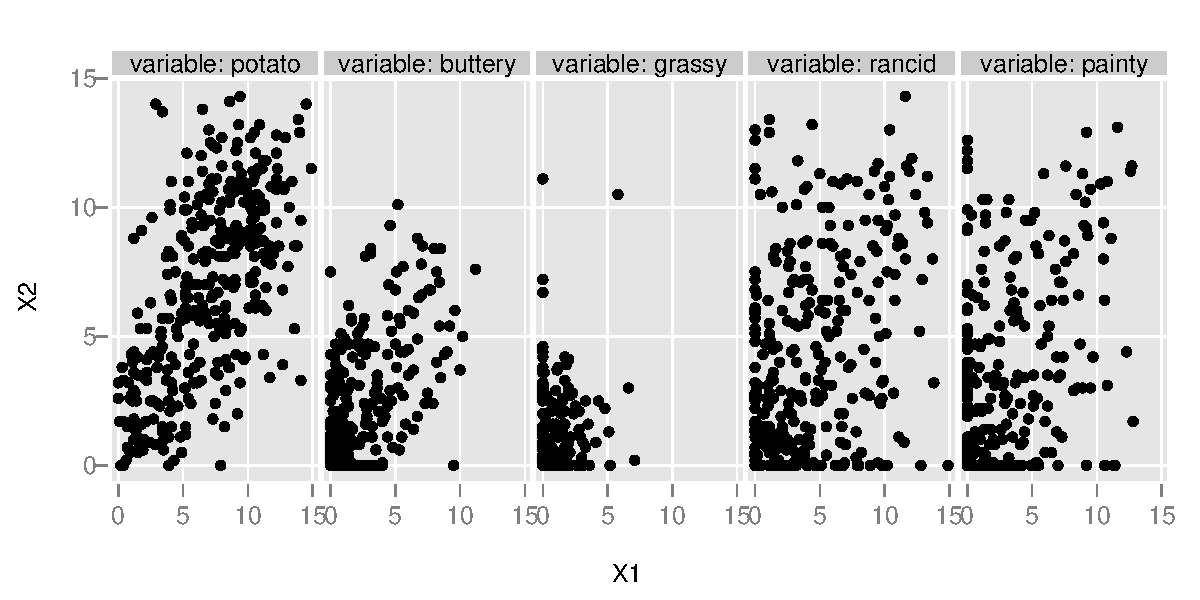
\includegraphics[scale=1]{./include/3416a75f4cea9109507cacd8e2f2aefc-001.pdf}
\begin{alltt}

\end{alltt}
% >>>

This plot is not easy to understand, as we are plotting two rather unusual variables.  Each point corresponds to one measurement for a given subject, date and time.  This gives a scatterplot for each variable that can be used to assess the inter-rep relationship.  The correlation looks strong for potatoey, weak for buttery and grassy, and particularly poor for painty.  This has a nice explanation: subjects were trained in tasting potatoey flavours, but not any of the others.

If we wanted to explore the relationships between subjects or times or treatments we could follow similar steps.

\newpage
\section{Where to go next}

Now that you've read this introduction, you should be able to get started using the {\tt reshape} package.  You can find a quick reference and more examples in {\tt ?melt} and {\tt ?cast}.   You can find some additional information on the reshape website \url{http://had.co.nz/reshape}, including the latest version of this document, as well as  copies of presentations and papers related to reshape.  

I would like to include more case studies of reshape in use.  If you have an interesting example, or there is something you are struggling with please let me know: \href{mailto:h.wickham@gmail.com}{h.wickham@gmail.com}.

\end{document}
